\chapter{कणों के निकाय; दृढ़ पिंडों का परिचय}\label{ch:b1:systems-of-points}

कोई गोताखोर तख़्ते से कूदती है, सिमटती है, दो कलाबाज़ियाँ खाती है और फिर
सीधी हो जाती है; इस सबके दौरान उसके शरीर का एक बिंदु --- उसका \omterm{def:b1:systems-of-points:cm}{द्रव्यमान
केंद्र} --- ठीक वही सादा परवलय खींचता है जो कोई पत्थर खींचता। हाथ से छोड़ा
गया कोई यो-यो अपनी डोरी के सिरे तक पहुँचने में पत्थर से तीन गुना समय लेता
है, और वहाँ दो हज़ार चक्कर प्रति मिनट से घूमता हुआ पहुँचता है। किसी भी ढाल
पर ठोस गोला खोखले गोले से जीत जाता है, चाहे उनके आकार या द्रव्यमान कुछ भी
हों। पिछले अध्यायों में चली आई एक बिंदु की यांत्रिकी कुछ ही प्रमेयों के
सहारे बहुत-से बिंदुओं के निकायों तक --- और रोज़मर्रा के दृढ़ पिंडों तक ---
फैल जाती है: \omterm{def:b1:systems-of-points:cm}{द्रव्यमान केंद्र} किसी बिंदु की तरह चलता है, ऊर्जा और \omterm{def:b1:angular-momentum:L}{कोणीय
संवेग} द्रव्यमान-केंद्र वाले भाग तथा उसके ``चारों ओर'' वाले भाग में बँट
जाते हैं, और किसी स्थिर अक्ष के परितः घूमता पिंड अपने \omterm{prop:b1:angular-momentum:inertia}{जड़त्व आघूर्ण} से
शासित एक ही स्वातंत्र्य-कोटि का निकाय होता है।

\section{द्रव्यमान केंद्र और संवेग}

\begin{definition}[द्रव्यमान केंद्र; निकाय का संवेग]\label{def:b1:systems-of-points:cm}
\index{द्रव्यमान केंद्र}\index{भारकेंद्र}
$m_i$ द्रव्यमानों के, $M_i$ पर स्थित कणों के लिए, जिनका कुल द्रव्यमान
$M = \sum m_i$ है, \emph{द्रव्यमान केंद्र} (भारकेंद्र) $G$ इस प्रकार
परिभाषित होता है
\[
\sum_i m_i\,\vect{GM_i} = \vect 0, \qquad\text{अर्थात्}\qquad
\vect{OG} = \frac{1}{M}\sum_i m_i\,\vect{OM_i}
\]
किसी भी मूलबिंदु $O$ के लिए। निकाय का \emph{संवेग} $\vect P =
\sum_i m_i\vect v_i = M\vect v_G$ है।
\end{definition}

\begin{theorem}[द्रव्यमान केंद्र की प्रमेय]\label{thm:b1:systems-of-points:cmtheorem}
\index{द्रव्यमान केंद्र की प्रमेय}\index{संवेग संरक्षण}
किसी \omterm{thm:b1:newton-dynamics:laws}{जड़त्वीय तंत्र} में,
\[
M\,\vect a_G = \frac{\dd\vect P}{\dd t} = \sum\vect F_{\mathrm{ext}} :
\]
यानी \omterm{def:b1:systems-of-points:cm}{द्रव्यमान केंद्र} $M$ द्रव्यमान के किसी \omterm{def:b1:point-kinematics:frame}{बिंदु कण} की तरह चलता है, जिस
पर केवल \emph{बाह्य} बलों का परिणामी लगता है। बिना किसी बाह्य बल वाले
\omterm{def:b1:newton-dynamics:conservation}{संवृत निकाय} के लिए $\vect P$ संरक्षित रहता है और $G$ एकसमान चलता है।
\end{theorem}

\begin{proof}
न्यूटन के दूसरे नियम को कणों पर जोड़ दीजिए; आंतरिक बल क्रिया--प्रतिक्रिया
युग्मों में कट जाते हैं; और $G$ की परिभाषा को दो बार अवकलित करने पर
$\sum m_i\vect a_i = M\vect a_G$।
\end{proof}

\begin{example}[गोताखोर, प्रतिक्षेप, संघट्ट]\label{ex:b1:systems-of-points:cm}
\index{संघट्ट}
गोताखोर का $G$ केवल उसके भार के अधीन परवलय पर चलता है, चाहे वह जैसे भी
मरोड़े --- उसकी माँसपेशियाँ आंतरिक बल हैं। \qty{4.0}{kg} की कोई राइफ़ल
\qty{10}{g} की गोली \qty{800}{m/s} से चलाती है: पहले और बाद में
$\vect P = \vect 0$, अतः राइफ़ल \qty{2.0}{m/s} से पीछे हटती है। दो कारें,
\qty{20}{m/s} पर \qty{1000}{kg} और विराम में \qty{1500}{kg}, जो टकराकर
आपस में फँस जाती हैं: $v =
20000/2500 = \qty{8.0}{m/s}$ --- संवेग संरक्षित, जबकि \omterm{thm:b1:work-and-energy:ke}{गतिज ऊर्जा} का
$60\%$ मुड़ी हुई धातु और ऊष्मा में चला गया। संवेग हर संघट्ट में संरक्षित
रहता है; \omterm{thm:b1:work-and-energy:ke}{गतिज ऊर्जा} केवल \emph{प्रत्यास्थ} संघट्टों में
(\cref{exo:b1:systems-of-points:12})।
\end{example}

\section{कोनिग की प्रमेयें}

\begin{definition}[भारकेंद्रीय तंत्र]\label{def:b1:systems-of-points:barycentric}
\index{भारकेंद्रीय तंत्र}
\emph{भारकेंद्रीय तंत्र} $\mathcal R^*$ का मूलबिंदु $G$ पर है और वह
\omterm{thm:b1:newton-dynamics:laws}{जड़त्वीय तंत्र} $\mathcal R$ के सापेक्ष स्थानांतरण में है (उसकी अक्षें
स्थिर दिशाएँ बनाए रखती हैं)। उसमें मापी गई राशियों पर तारांकन लगाया जाता
है: $\vect v_i^*
= \vect v_i - \vect v_G$, और $\sum m_i\vect v_i^* = \vect 0$।
\end{definition}

\begin{theorem}[कोनिग की प्रमेयें]\label{thm:b1:systems-of-points:koenig}
\index{कोनिग की प्रमेयें}
किसी निकाय का, किसी बिंदु $O$ के परितः, \omterm{def:b1:angular-momentum:L}{कोणीय संवेग} और उसकी \omterm{thm:b1:work-and-energy:ke}{गतिज ऊर्जा} दो
भागों में बँट जाते हैं: पूरा द्रव्यमान लिए हुए उसके \omterm{def:b1:systems-of-points:cm}{द्रव्यमान केंद्र} का
योगदान, और \omterm{def:b1:systems-of-points:barycentric}{भारकेंद्रीय तंत्र} में के योगदान:
\[
\vect L_O = \vect{OG}\wedge M\vect v_G + \vect L^*, \qquad
E_k = \tfrac12 Mv_G^2 + E_k^*,
\]
जहाँ $\vect L^* = \sum\vect{GM_i}\wedge m_i\vect v_i^*$ और $E_k^* = \sum\tfrac12
m_iv_i^{*2}$ तंत्र के मूलबिंदु पर निर्भर नहीं करते।
\end{theorem}

\begin{proof}
$\vect{OM_i} = \vect{OG} + \vect{GM_i}$ और $\vect v_i = \vect v_G + \vect v_i^*$;
$\sum\vect{OM_i}\wedge m_i\vect v_i$ और $\sum\tfrac12 m_iv_i^2$ को फैलाइए: मिश्रित
पदों में $\sum m_i\vect{GM_i} = \vect 0$ या $\sum m_i\vect v_i^* = \vect 0$
आ जाता है और वे लुप्त हो जाते हैं।
\end{proof}

\begin{example}[लुढ़कता पहिया]\label{ex:b1:systems-of-points:rolling}
\index{बिना फिसले लुढ़कना}
$M$ द्रव्यमान, $R$ त्रिज्या और अपनी धुरी के परितः $J$ \omterm{prop:b1:angular-momentum:inertia}{जड़त्व आघूर्ण} वाला
कोई पहिया $v$ चाल से बिना फिसले लुढ़क रहा है: संस्पर्श बिंदु विराम में है,
अतः $\omega = v/R$, और $E_k = \tfrac12 Mv^2 + \tfrac12 J\omega^2 = \tfrac12 Mv^2(1 +
J/MR^2)$ --- यानी एकसमान चकती के लिए $Mv^2$ का तीन-चौथाई ($J = \tfrac12 MR^2$),
और छल्ले के लिए पूरा $Mv^2$। दूसरा पद ही वह कारण है जिससे साइकिल के पहिये
हलके बनाए जाते हैं: उनके घूर्णन में वह ऊर्जा लगती है जो ढाँचे के द्रव्यमान
में नहीं लगती।
\end{example}

\section{द्वि-पिंड समस्या}

\begin{proposition}[समानीत द्रव्यमान]\label{prop:b1:systems-of-points:twobody}
\index{द्वि-पिंड समस्या}\index{समानीत द्रव्यमान}
केवल आपस में अन्योन्यक्रिया करते दो कण (बल $\vect F$ जो $m_2$ पर $m_1$ से
लगता है, और $-\vect F$ जो $m_1$ पर): $G$ एकसमान चलता है, और सापेक्ष स्थिति
$\vect r = \vect{M_1M_2}$ इस नियम का पालन करती है
\[
\mu\,\frac{\dd^2\vect r}{\dd t^2} = \vect F, \qquad \mu = \frac{m_1m_2}{m_1 + m_2},
\]
यानी \emph{\omterm{prop:b1:systems-of-points:twobody}{समानीत द्रव्यमान}} $\mu$ के किसी एक काल्पनिक कण का समीकरण, जो
किसी स्थिर केंद्र के परितः $\vect F$ के अधीन चल रहा हो। $\mathcal R^*$ में, $E_k^* =
\tfrac12\mu\dot{\vect r}^2$ और $\vect L^* = \vect r\wedge\mu\dot{\vect r}$।
\end{proposition}

\begin{proof}
$\ddot{\vect r} = \vect a_2 - \vect a_1 = \vect F/m_2 + \vect F/m_1 = \vect F(m_1 +
m_2)/m_1m_2$। $\mathcal R^*$ में, $\vect{GM_2} = m_1\vect r/(m_1 + m_2)$ और
$\vect{GM_1} = -m_2\vect r/(m_1 + m_2)$; इन्हें $E_k^*$ और $\vect L^*$ में रखिए।
\end{proof}

\begin{example}[जब केंद्र भी चलता है]\label{ex:b1:systems-of-points:reduced}
\cref{ch:b1:central-forces} में सूर्य स्थिर था: यह केवल
$m \ll M$ की सीमा में यथार्थ है; सामान्यतः \omterm{thm:b1:central-forces:circular}{केप्लर का तीसरा नियम} $T^2 = 4\pi^2a^3/G(M +
m)$ कहता है। \cref{pb:b1:work-and-energy:1} के कंपमान हाइड्रोजन
क्लोराइड अणु के लिए,
कूप में दोलन करता द्रव्यमान $\mu = m_Hm_{Cl}/(m_H + m_{Cl}) =
0.972\,m_H$ है, जो आवृत्ति को $1.4\%$ बढ़ा देता है; और हाइड्रोजन परमाणु
के लिए इलेक्ट्रॉन का $\mu$, $m_e$ से $1836$ में एक भाग जितना भिन्न है ---
जो वर्णक्रम में मापा जा सकता है।
\end{example}

\section{स्थिर अक्ष के परितः घूमता दृढ़ पिंड}

\begin{definition}[दृढ़ पिंड; स्थिर अक्ष के परितः घूर्णन]\label{def:b1:systems-of-points:solid}
\index{दृढ़ पिंड}\index{स्थिर अक्ष के परितः घूर्णन}
\emph{दृढ़ पिंड} (ठोस) ऐसा निकाय है जिसके बिंदु आपसी दूरियाँ स्थिर रखते
हैं। यदि वह तंत्र में स्थिर किसी अक्ष $\Delta$ के परितः घूमे, तो उसका हर
बिंदु $\Delta$ पर केंद्रित कोई वृत्त खींचता है, और सब एक ही \omterm{cor:b1:point-kinematics:circular}{कोणीय वेग}
$\omega = \dot\theta$ से; अक्ष से $r_i$ दूरी पर के बिंदु की चाल
$r_i\omega$ होती है।
\end{definition}

\begin{proposition}[जड़त्व आघूर्ण; कोणीय संवेग; गतिज ऊर्जा]\label{prop:b1:systems-of-points:inertia}
\index{जड़त्व आघूर्ण!ठोसों का}\index{ह्यूगेंस की प्रमेय}
\emph{\omterm{prop:b1:angular-momentum:inertia}{जड़त्व आघूर्ण}} $J_\Delta = \sum m_ir_i^2$ के साथ (संतत पिंड के लिए
समाकल $\int r^2\,\dd m$):
\[
L_\Delta = J_\Delta\,\omega, \qquad E_k = \tfrac12 J_\Delta\omega^2 .
\]
मानक मान (द्रव्यमान $M$): पतला छल्ला या खोखला बेलन अपनी अक्ष के परितः,
$MR^2$; एकसमान चकती या ठोस बेलन, $\tfrac12 MR^2$; $L$ लंबाई की पतली छड़
अपने केंद्र के परितः, $\tfrac{1}{12}ML^2$, और एक सिरे के परितः,
$\tfrac13 ML^2$; ठोस गोला किसी व्यास के परितः, $\tfrac25 MR^2$।
\emph{\omterm{prop:b1:systems-of-points:inertia}{ह्यूगेंस की प्रमेय}}: ऐसी किसी अक्ष $\Delta$ के परितः जो अक्ष
$\Delta_G$ के समांतर हो और $G$ से जाती उस अक्ष से $d$ दूरी पर हो, $J_\Delta = J_{\Delta_G} + Md^2$।
\end{proposition}

\begin{proof}
$L_\Delta$ और $E_k$: \cref{prop:b1:angular-momentum:inertia}। छड़, उसके
सिरे के परितः: $\int_0^L x^2(M/L)\,\dd x = ML^2/3$; और केंद्र के परितः, $\int_{-L/2}^{L/2}
x^2(M/L)\dd x = ML^2/12$। चकती: $r$ त्रिज्या, $\dd r$ चौड़ाई और
$(2Mr/R^2)\dd r$ द्रव्यमान का छल्ला: $\int_0^R r^2(2Mr/R^2)\dd r = MR^2/2$; छल्ला और
गोला स्वीकृत मान लिए गए हैं (गोले के लिए द्विसमाकल चाहिए)। ह्यूगेंस:
$r_i^2 = \abs{\vect{GM_i}_\perp + \vect d}^2 = r_{G,i}^2 + d^2 + 2\vect d\cdot
\vect{GM_i}_\perp$ के साथ, मिश्रित पद $G$ की परिभाषा से शून्य पर जुड़ जाता है।
\end{proof}

\begin{omfigure}
\begin{tikzpicture}[font=\small, x=1cm, y=1cm]
  % disk with ring element
  \draw[omDef, thick, fill=omDef!8] (0,0) circle (1.8);
  \draw[omDef!70, fill=omDef!35] (0,0) circle (1.15); \draw[omDef!70, fill=omDef!8] (0,0) circle (1.0);
  \fill (0,0) circle (1.2pt);
  \draw[-Stealth] (0,0) -- (30:1.07) node[midway, above left, font=\footnotesize] {$r$};
  \node[font=\footnotesize] at (30:1.55) {$\dd r$};
  \node[omDef, font=\footnotesize] at (0,-2.3) {$J = \int r^2\,\dd m = \tfrac12 MR^2$};
  % Huygens
  \begin{scope}[xshift=6.2cm]
  \draw[omThm, thick, fill=omThm!8] (0,0) circle (1.6);
  \fill (0,0) circle (1.5pt) node[below] {$G$};
  \fill[omThm] (1.6,0) circle (1.8pt) node[right] {$\Delta$};
  \draw[Stealth-Stealth] (0,0.3) -- (1.6,0.3) node[midway, above] {$d$};
  \node[omThm, font=\footnotesize] at (0,-2.3) {$J_\Delta = J_{\Delta_G} + Md^2 = \tfrac32 MR^2$};
  \end{scope}
\end{tikzpicture}

{\small बाएँ: किसी चकती का \omterm{prop:b1:angular-momentum:inertia}{जड़त्व आघूर्ण}, छल्ले-दर-छल्ला जोड़ा हुआ। दाएँ:
\omterm{prop:b1:systems-of-points:inertia}{ह्यूगेंस की प्रमेय} --- किसी चकती के किनारे से जाती उस अक्ष के परितः जो
उसके केंद्र से जाती अक्ष के समांतर है, $J = \tfrac12 MR^2 + MR^2$।}
\end{omfigure}

\begin{theorem}[स्थिर अक्ष के परितः किसी ठोस की गतिकी]\label{thm:b1:systems-of-points:rotation}
\index{धुरी}\index{आघूर्ण की शक्ति}
किसी \omterm{thm:b1:newton-dynamics:laws}{जड़त्वीय तंत्र} में स्थिर अक्ष $\Delta$ के परितः घूमते किसी ठोस के लिए,
\[
J_\Delta\,\ddot\theta = \sum\mathcal M_\Delta(\vect F_{\mathrm{ext}}),
\qquad
\frac{\dd}{\dd t}\Big(\tfrac12 J_\Delta\dot\theta^2\Big) = \sum\mathcal M_\Delta(\vect F_{\mathrm{ext}})\,\dot\theta :
\]
यानी अक्ष के परितः बाह्य बलों के आघूर्ण ही कोणीय त्वरण चलाते हैं, और कोई
आघूर्ण $\mathcal M_\Delta$ शक्ति
$\mathcal M_\Delta\omega$ देता है। कोई आदर्श \emph{धुरी} (घर्षणरहित धारक) अपनी अक्ष
के परितः कोई आघूर्ण नहीं लगाती, अतः वह घूर्णन को न तेज़ करती है न
रोकती है।
\end{theorem}

\begin{proof}
\cref{thm:b1:angular-momentum:system} को $\Delta$ पर प्रक्षेपित कीजिए, जहाँ $L_\Delta
= J_\Delta\dot\theta$ है और \omterm{def:b1:systems-of-points:solid}{दृढ़ पिंड} के लिए $J_\Delta$ अचर; ऊर्जा वाले रूप के
लिए $\dot\theta$ से गुणा कीजिए (\omterm{def:b1:systems-of-points:solid}{दृढ़ पिंड} के आंतरिक बल कोई कार्य नहीं
करते: दूरियाँ बदलती ही नहीं)।
\end{proof}

\begin{example}[संयुक्त लोलक; ऐंठन लोलक]\label{ex:b1:systems-of-points:pendulums}
\index{संयुक्त लोलक}\index{ऐंठन लोलक}
$M$ द्रव्यमान का कोई ठोस किसी क्षैतिज अक्ष के परितः धुरी पर घूमता है,
जिसकी दूरी $d$ \omterm{def:b1:systems-of-points:cm}{द्रव्यमान केंद्र} $G$ से नापी जाती है: भार का आघूर्ण
$-Mgd\sin\theta$ है, अतः $J_\Delta\ddot\theta =
-Mgd\sin\theta$, और छोटे झूलों का आवर्तकाल यह होता है
\[
T = 2\pi\sqrt{\frac{J_\Delta}{Mgd}} ,
\]
यानी $J_\Delta/Md$ लंबाई के किसी \omterm{ex:b1:newton-dynamics:pendulum}{सरल लोलक} का आवर्तकाल --- एक सिरे पर धुरी
वाली एकसमान छड़ के लिए $2L/3$। ऐंठन नियतांक
$C$ वाले किसी तार से लटकी चकती (प्रत्यानयन आघूर्ण $-C\theta$): $J\ddot\theta = -C\theta$, $T = 2\pi\sqrt{J/C}$
--- यही वह ऐंठन तुला है जिसने $G$ और कूलॉम का नियम मापा।
\end{example}

\begin{omfigure}
\begin{tikzpicture}[font=\small, x=1cm, y=1cm]
  % compound pendulum: plate pivoted at top
  \fill[pattern=north east lines] (-0.8,3.4) rectangle (0.8,3.6); \draw[thick] (-0.8,3.4) -- (0.8,3.4);
  \fill (0,3.3) circle (1.6pt);
  \begin{scope}[rotate around={-20:(0,3.3)}]
    \draw[thick, fill=omDef!12] (-0.5,0.3) rectangle (0.5,3.3);
    \fill (0,1.7) circle (1.6pt); \node[right] at (0.05,1.7) {$G$};
    \draw[-Stealth, omThm, very thick] (0,1.7) -- ++(0,-1.4);
  \end{scope}
  \draw[dashed] (0,3.3) -- (0,0.4);
  \node[omThm] at (0.75,0.55) {$M\vect g$};
  \draw (0,2.3) arc (-90:-110:1.0); \node at (-0.3,2.1) {$\theta$};
  \node[font=\footnotesize] at (0,-0.1) {$T = 2\pi\sqrt{J_\Delta/Mgd}$};
  % torsion pendulum
  \begin{scope}[xshift=5.5cm]
  \fill[pattern=north east lines] (-0.8,3.4) rectangle (0.8,3.6); \draw[thick] (-0.8,3.4) -- (0.8,3.4);
  \draw[thick] (0,3.4) -- (0,1.6);
  \draw[omDef, thick, fill=omDef!12] (0,1.3) ellipse (1.4 and 0.35);
  \draw[-Stealth, omProp, thick] (0.9,1.05) arc (-60:30:0.9) node[right] {$\theta$};
  \node[font=\footnotesize] at (0,-0.1) {$T = 2\pi\sqrt{J/C}$};
  \end{scope}
  % rolling down incline
  \begin{scope}[xshift=10.2cm]
  \draw[thick] (-1.6,0) -- (2.4,0) -- (-1.6,2.2) -- cycle;
  \draw[omThm, thick, fill=omThm!10] ($(-0.6,1.65)+(61.2:0.5)$) circle (0.5);
  \draw[-Stealth, omThm, thick] ($(-0.6,1.65)+(61.2:0.5)$) -- ++(-28.8:1.1) node[below right] {$\vect v_G$};
  \node[font=\footnotesize] at (0.5,-0.35) {$a = \dfrac{g\sin\alpha}{1 + J/MR^2}$};
  \draw (1.6,0) arc (180:151.2:0.8); \node at (1.35,0.25) {$\alpha$};
  \end{scope}
\end{tikzpicture}

{\small गति में तीन ठोस: किसी धुरी के परितः झूलता \omterm{ex:b1:systems-of-points:pendulums}{संयुक्त लोलक} (अक्ष के
परितः भार का आघूर्ण), कोई \omterm{ex:b1:systems-of-points:pendulums}{ऐंठन लोलक} (तार का आघूर्ण), और किसी ढाल पर बिना
फिसले लुढ़कता कोई ठोस --- उसका $J/MR^2$ जितना बड़ा, वह उतना ही धीरे
लुढ़कता है।}
\end{omfigure}

\begin{proposition}[ढाल पर बिना फिसले लुढ़कना]\label{prop:b1:systems-of-points:rollingincline}
कोई घूर्णज ठोस (अपनी अक्ष के परितः $J = kMR^2$), जिसे $\alpha$ कोण की किसी
ढाल पर छोड़ा गया हो, इस त्वरण से बिना फिसले लुढ़कता है
\[
a = \frac{g\sin\alpha}{1 + k} :
\]
ठोस गोले के लिए $\tfrac57 g\sin\alpha$, चकती के लिए $\tfrac23 g\sin\alpha$,
और छल्ले के लिए $\tfrac12 g\sin\alpha$ --- द्रव्यमान और त्रिज्या से स्वतंत्र।
\end{proposition}

\begin{proof}
ऊर्जा: ढाल के अनुदिश $Mgh = \tfrac12 Mv^2(1 + k)$ (विराम में पड़े संस्पर्श
बिंदु पर स्थैतिक घर्षण कोई कार्य नहीं करता), अतः $v^2 = 2ah$, जहाँ $a$ ऊपर
दिया हुआ है; अथवा $G$ के लिए न्यूटन और $G$ के परितः आघूर्ण प्रमेय, घर्षण
$f$ के साथ: $Ma = Mg\sin\alpha - f$, $kMR^2\dot\omega = fR$, $a = R\dot\omega$।
\end{proof}

\begin{remark}[विरूप्य निकाय]\label{rem:b1:systems-of-points:deformable}
\index{विरूप्य निकाय}
जो निकाय दृढ़ नहीं है, उसके लिए \omterm{thm:b1:work-and-energy:ke}{गतिज ऊर्जा} प्रमेय यह कहती है:
$\Delta E_k = W_{\mathrm{ext}} + W_{\mathrm{int}}$, यानी आंतरिक बल भी कार्य
करते हैं (माँसपेशियाँ, स्प्रिंग, निकाय के भीतर का घर्षण)। बाँहें भीतर
खींचती स्केटर, सिमटती गोताखोर, पैडलों पर खड़ा साइकिल-सवार --- सब बिना किसी
बाह्य कार्य के \omterm{thm:b1:work-and-energy:ke}{गतिज ऊर्जा} पा लेते हैं; \omterm{thm:b1:systems-of-points:cmtheorem}{द्रव्यमान केंद्र की प्रमेय} सच बनी
रहती है, और ऊर्जा भीतर से आती है।
\end{remark}

\section{अभ्यास}

\begin{exercise}[$\star$]\label{exo:b1:systems-of-points:1}
$x = 0$ पर \qty{2.0}{kg} और $x = \qty{1.0}{m}$ पर \qty{3.0}{kg} द्रव्यमान:
$G$ की स्थिति। पृथ्वी--चंद्र निकाय ($81:1$, \qty{384000}{km}): पृथ्वी के
केंद्र से $G$ की दूरी; पृथ्वी की त्रिज्या से उसकी तुलना
कीजिए।
\end{exercise}

\begin{exercise}[$\star$]\label{exo:b1:systems-of-points:2}
\qty{4.0}{kg} की कोई राइफ़ल \qty{10}{g} की गोली \qty{800}{m/s} से चलाती
है। प्रतिक्षेप चाल; गोली और राइफ़ल की गतिज ऊर्जाएँ; और वह ऊर्जा आई कहाँ
से?
\end{exercise}

\begin{exercise}[$\star$]\label{exo:b1:systems-of-points:3}
\qty{20}{m/s} पर चलती \qty{1000}{kg} की कोई कार विराम में खड़ी
\qty{1500}{kg} की कार से टकराकर उससे फँस जाती है। उभयनिष्ठ चाल; \omterm{thm:b1:work-and-energy:ke}{गतिज ऊर्जा} का खोया हुआ अंश।
\end{exercise}

\begin{exercise}[$\star$]\label{exo:b1:systems-of-points:4}
$M$ द्रव्यमान और $L$ लंबाई की किसी एकसमान छड़ का \omterm{prop:b1:angular-momentum:inertia}{जड़त्व आघूर्ण} उसके सिरे
से जाती लंब अक्ष के परितः व्युत्पन्न कीजिए, फिर केंद्र से जाती अक्ष के
परितः; और दोनों के बीच \omterm{prop:b1:systems-of-points:inertia}{ह्यूगेंस की प्रमेय} जाँचिए।
\end{exercise}

\begin{exercise}[$\star\star$]\label{exo:b1:systems-of-points:5}
एक ही द्रव्यमान और चाल वाले, लुढ़कते एकसमान बेलन और लुढ़कते छल्ले की \omterm{thm:b1:work-and-energy:ke}{गतिज
ऊर्जा}, $\tfrac12 Mv^2$ के गुणजों में। खुरदरे समतल फ़र्श पर कौन पहले
रुकता है, और किसी ढाल पर कौन अधिक ऊँचा चढ़ता है?
\end{exercise}

\begin{exercise}[$\star\star$]\label{exo:b1:systems-of-points:6}
हाइड्रोजन क्लोराइड ($m_{Cl} = 35m_H$) का और हाइड्रोजन परमाणु
($m_p = 1836m_e$) का \omterm{prop:b1:systems-of-points:twobody}{समानीत द्रव्यमान}; और केवल हलके द्रव्यमान से निकाली
गई कंपन या कक्षीय आवृत्ति में सापेक्ष संशोधन।
\end{exercise}

\begin{exercise}[$\star\star$]\label{exo:b1:systems-of-points:7}
\qty{1.0}{m} लंबी कोई एकसमान छड़ एक सिरे के परितः स्वतंत्र रूप से धुरी पर
घूमती है। छोटे दोलनों का आवर्तकाल; उसी आवर्तकाल वाले \omterm{ex:b1:newton-dynamics:pendulum}{सरल लोलक} की लंबाई;
छड़ का वह बिंदु (आघात-केंद्र), जहाँ तेज़ प्रहार धुरी पर कोई प्रतिक्रिया
नहीं देता, उसी दूरी पर होता है --- बल्लेबाज़ उसे क्यों ढूँढ़ता है?
\end{exercise}

\begin{exercise}[$\star\star$]\label{exo:b1:systems-of-points:8}
कोई चकती ($M = \qty{0.20}{kg}$, $R = \qty{10}{cm}$) किसी तार से लटकी है और
\qty{2.0}{s} आवर्तकाल से ऐंठन में दोलन करती है। तार का ऐंठन नियतांक
निकालिए।
\end{exercise}

\begin{exercise}[$\star\star$]\label{exo:b1:systems-of-points:9}
\qty{10}{kg.m^2} \omterm{prop:b1:angular-momentum:inertia}{जड़त्व आघूर्ण} का कोई जड़त्व चक्र \qty{3000}{rpm} से घूमता
है। संचित ऊर्जा; उसे \qty{10}{s} में रोक देने वाला ब्रेक-आघूर्ण; और ब्रेक
लगने के दौरान चक्करों की संख्या।
\end{exercise}

\begin{exercise}[$\star\star\star$]\label{exo:b1:systems-of-points:10}
कोई ठोस गोला, कोई ठोस बेलन और कोई छल्ला किसी ढाल के शिखर से एक साथ छोड़े
जाते हैं। पहुँचने का क्रम, और उनके त्वरणों का अनुपात। क्या परिणाम उनकी
त्रिज्याओं या द्रव्यमानों पर निर्भर करता है?
\end{exercise}

\begin{exercise}[$\star\star\star$]\label{exo:b1:systems-of-points:11}
प्रक्षेप्य लोलक: \qty{400}{m/s} की \qty{10}{g} गोली \qty{1.0}{m} डोरी से
लटके \qty{2.0}{kg} के गुटके में धँस जाती है। टक्कर के ठीक बाद की चाल;
पहुँची हुई ऊँचाई; गोली की \omterm{thm:b1:work-and-energy:ke}{गतिज ऊर्जा} का खोया हुआ अंश। टक्कर के लिए ही
ऊर्जा संरक्षण क्यों नहीं लगाया जा सकता?
\end{exercise}

\begin{exercise}[$\star\star\star$]\label{exo:b1:systems-of-points:12}
$m_1$, जो $v_1$ चाल से चल रहा है, का विराम में पड़े $m_2$ से आमने-सामने
प्रत्यास्थ संघट्ट:
$v_1' = \frac{m_1 - m_2}{m_1 + m_2}v_1$ और $v_2' = \frac{2m_1}{m_1 + m_2}v_1$
व्युत्पन्न कीजिए। कोई न्यूट्रॉन जब किसी प्रोटॉन से टकराता है, किसी कार्बन
नाभिक ($12m_n$) से, और किसी सीसा नाभिक ($207m_n$) से, तो हस्तांतरित ऊर्जा
का अंश। रिएक्टरों में मंदन हलके नाभिकों से क्यों किया जाता है?
\end{exercise}

\begin{omfigure}
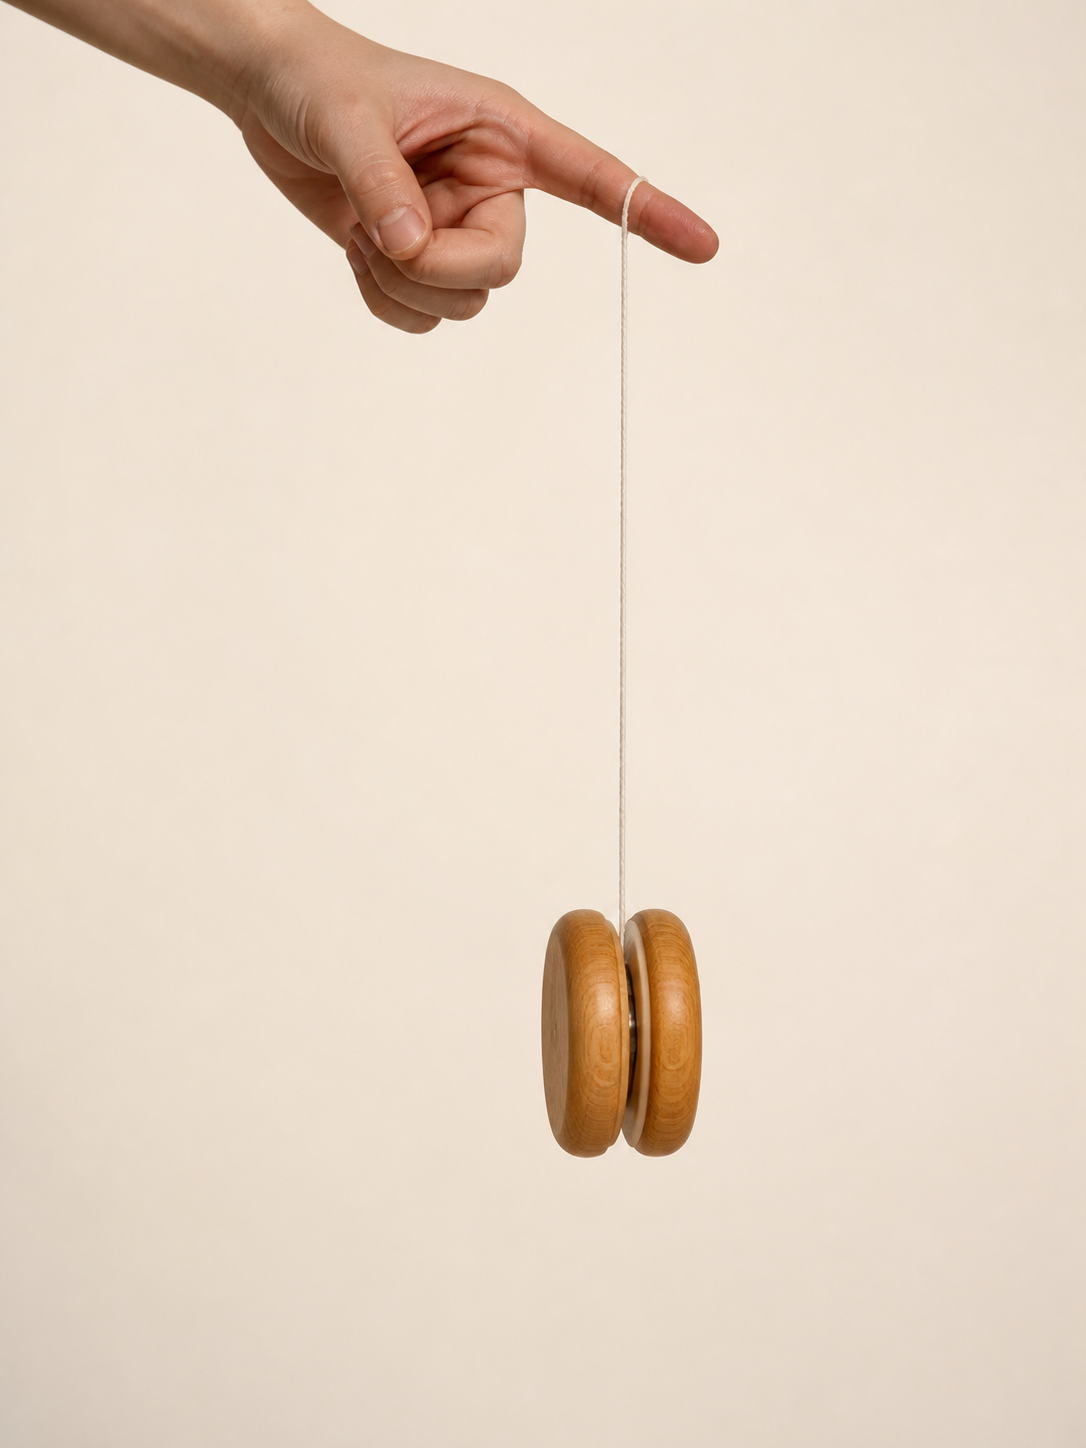
\includegraphics[width=0.34\linewidth]{images/book3/ai/b3-19-yoyo-unwinding.png}

{\small खुलता हुआ यो-यो: \omterm{def:b1:systems-of-points:cm}{द्रव्यमान केंद्र} गिरता है, चकती घूमती है, और डोरी का तनाव ही वह है जो दोनों गतियों को आपस में बाँधता है --- यही सप्ताहांत समस्या है।}
\end{omfigure}

\section{समस्या: यो-यो}

\begin{problem}[{सप्ताहांत समस्या --- डोरी के सिरे पर पतली धुरी वाली एक
चकती: वह इतनी धीरे क्यों गिरती है, तली पर कितनी तेज़ी से घूमती है, वहाँ
``सोती'' क्यों है, और धागा खींचने पर कोई फिरकी किस ओर
लुढ़कती है}]
\label{pb:b1:systems-of-points:1}
यो-यो $M = \qty{50}{g}$ द्रव्यमान और $R =
\qty{3.0}{cm}$ त्रिज्या की एकसमान चकती है, जिसमें $r = \qty{0.40}{cm}$
त्रिज्या की एक पतली धुरी है और उस पर $h = \qty{1.0}{m}$ लंबी डोरी लिपटी
है; डोरी का ऊपरी सिरा स्थिर पकड़ा गया है। $g = \qty{9.81}{m/s^2}$; अक्ष के
परितः $J = \tfrac12 MR^2$।

\medskip
\noindent\textbf{भाग I --- शुद्धगतिकी और ऊर्जा।}
\begin{enumerate}
  \item यो-यो का \omterm{def:b1:systems-of-points:cm}{द्रव्यमान केंद्र} $G$ कहाँ है? क्यों?
  \item कोनिग की प्रमेय से दिखाइए कि उसकी \omterm{thm:b1:work-and-energy:ke}{गतिज ऊर्जा} $\tfrac12
        Mv_G^2 + \tfrac12 J\omega^2$ है।
  \item छल्लों पर समाकलित करके $J = \tfrac12 MR^2$ व्युत्पन्न कीजिए, और
        $J$ का मान निकालिए।
  \item डोरी धुरी से बिना फिसले खुलती है: इससे $v_G$ और $\omega$ के बीच
        संबंध जोड़िए।
  \item इससे $E_k = \tfrac12 Mv_G^2(1 + R^2/2r^2)$ निकालिए और कोष्ठक वाला
        गुणक गिनिए। टिप्पणी कीजिए।
\end{enumerate}

\medskip
\noindent\textbf{भाग II --- गिरना।}
\begin{enumerate}[resume]
  \item यो-यो पर लगने वाले बल; \omterm{thm:b1:systems-of-points:cmtheorem}{द्रव्यमान केंद्र की प्रमेय} लिखिए
        (ऊर्ध्वाधर अक्ष नीचे की ओर)।
  \item $G$ से जाती अक्ष के परितः \omterm{def:b1:angular-momentum:L}{कोणीय संवेग} की प्रमेय लिखिए (किन बलों
        का आघूर्ण है?)।
  \item प्रश्न 4 के साथ मिलाकर त्वरण $a_G = g/(1 +
        R^2/2r^2)$ निकालिए; और उसका मान गिनिए।
  \item डोरी का तनाव निकालिए और भार से तुलना कीजिए।
  \item \qty{1.0}{m} डोरी के खुलने में लगा समय, और तब की चाल; उसी ऊँचाई
        से गिराए गए पत्थर से तुलना कीजिए।
  \item तली पर \omterm{cor:b1:point-kinematics:circular}{कोणीय वेग}, रेडियन प्रति सेकंड में और चक्कर प्रति मिनट में।
  \item तली पर \omterm{thm:b1:work-and-energy:ke}{गतिज ऊर्जा} को उसके स्थानांतरी और घूर्णी भागों में बाँटिए।
  \item ऊर्जा-संतुलन जाँचिए: $Mgh$ की तली पर की \omterm{thm:b1:work-and-energy:ke}{गतिज ऊर्जा} से तुलना
        कीजिए, और बताइए कि डोरी का तनाव, बड़ा होते हुए भी, कोई कार्य
        क्यों नहीं करता।
\end{enumerate}

\medskip
\noindent\textbf{भाग III --- तली पर: सोता यो-यो।}
जब डोरी पूरी खुल जाती है तो वह \omterm{def:b1:systems-of-points:cm}{द्रव्यमान केंद्र} को कुछ ही मिलीसेकंड में
रोक देती है; यो-यो डोरी के सिरे के फंदे में घूमता रहता है (``सोना'')।
\begin{enumerate}[resume]
  \item $G$ के रुक जाने पर भी घूर्णन क्यों बचा रहता है? (कौन-सी प्रमेय,
        और उसे रोकने के लिए कौन-सा बल चाहिए होता?)
  \item यदि $G$ \qty{5}{ms} में रोक दिया जाए, तो रुकने के दौरान औसत तनाव
        आँकिए।
  \item फंदा धुरी पर घर्षण आघूर्ण $\Gamma =
        \qty{1.0e-4}{N.m}$ से रगड़ता है: यो-यो कितनी देर सोता है?
  \item डोरी पर ऊपर की ओर तेज़ झटका देने से डोरी फिर धुरी को पकड़ लेती
        है; तब घूमता यो-यो ऊपर चढ़ने लगता है। ऊर्जा से निकालिए: यदि कुछ
        भी न खोता, तो वह कितनी ऊँचाई तक उठ सकता? और व्यवहार में उससे कम
        क्यों?
  \item चढ़ने के दौरान तनाव भार से बड़ा होता है या छोटा? ($a_G$ का
        चिह्न।)
  \item यदि किसी यो-यो की धुरी की त्रिज्या $R$ के बराबर होती (डोरी किनारे
        पर लिपटी), तो क्या होता? उसका गिरने का त्वरण निकालिए।
\end{enumerate}

\medskip
\noindent\textbf{भाग IV --- मेज़ पर की फिरकी।}
वही वस्तु किसी खुरदरी मेज़ पर पड़ी है, धुरी क्षैतिज, और उसकी डोरी धुरी के
\emph{नीचे} से क्षैतिज दिशा में निकलती है; उसे $F$ बल से खींचा जाता है। वह
बिना फिसले लुढ़कती है।
\begin{enumerate}[resume]
  \item मेज़ के साथ संस्पर्श बिंदु $C$ पर फिरकी के पदार्थ का वेग क्या है?
        इससे निकालिए कि गति हर क्षण $C$ के परितः एक घूर्णन है।
  \item $F$ का आघूर्ण $C$ के परितः निकालिए (\omterm{def:b1:angular-momentum:moment}{उत्तोलक भुजा} $R - r$), और वही
        भार तथा मेज़ की प्रतिक्रिया के लिए।
  \item $C$ के परितः \omterm{def:b1:angular-momentum:L}{कोणीय संवेग} की प्रमेय, $J_C = J +
        MR^2$ (ह्यूगेंस) के साथ लगाकर, $a_G$ निकालिए और दिखाइए कि फिरकी
        हाथ की \emph{ओर} लुढ़कती है।
  \item अब डोरी क्षैतिज से $\beta$ कोण ऊपर की ओर खींची जाती है। दिखाइए कि
        जब $F$ की क्रिया-रेखा $C$ से होकर जाती है, अर्थात्
        $\cos\beta = r/R$, तब फिरकी लुढ़कती ही नहीं, और उससे अधिक खड़ी
        खिंचाई पर वह हाथ से दूर लुढ़कती है। वह कोण निकालिए।
  \item $a_G$ निकालिए, जब $F = \qty{0.20}{N}$ क्षैतिज दिशा में खींचा जाए,
        और आवश्यक घर्षण बल भी; फिरकी के फिसलने से पहले $F$ को कौन सीमित
        करता है?
  \item सार दीजिए: प्रयुक्त तीनों प्रमेयें (\omterm{def:b1:systems-of-points:cm}{द्रव्यमान केंद्र}, किसी अक्ष
        के परितः \omterm{def:b1:angular-momentum:L}{कोणीय संवेग}, ऊर्जा) और हर एक ने क्या तय किया।
\end{enumerate}
\end{problem}
